\newcommand{\doctitle}{Construct and Destroy \\ Software Architecture}
\newcommand{\doctitleshort}{C\&D Software Architecture}

\newcommand{\docauthor} {
    \renewcommand{\arraystretch}{0.5}
    \begin{tabular}{l l}
        \textbf{Students:} & ~ \\
        Mark van der Woude     & {\mdseries(S1081655)} \\
        Stephan Schrijver     & {\mdseries(S1078783)} \\
        Jeroen Vinke     & {\mdseries(S1078666)} \\
        Sander Bouwman   & {\mdseries(S1080528)} \\
        Robin T. Koning  & {\mdseries(S1078710)} \\
    \end{tabular}
}

\newcommand{\doctitlepage} {
    \thispagestyle{empty}
    \parbox[t]{1.0\linewidth}{
        \fontsize{40pt}{60pt}\selectfont
        \vspace*{1.5cm}
        \doctitle{}
        \vspace*{1.5cm}
    }
    \vfill
    {
        \centering
        \large
        \hfill \today
        \hfill \docauthor{}
    }
    \normalcolor{}

    \newpage
}

\providecommand{\doctitle}{Title}
\providecommand{\docauthor}{Author}
\providecommand{\doctype}{scrartcl}
\providecommand{\doctitlepage}{TitlePage}

\documentclass[12pt,a4paper,titlepage,parskip=full]{\doctype}

\usepackage[english]{babel}
\usepackage{caption}
\usepackage{float}
\usepackage{blindtext}
\usepackage{hyperref}
\usepackage{graphicx}
\usepackage{listings}
\usepackage{tikz}
\usetikzlibrary{decorations.pathreplacing}
\usepackage{pdfpages}
\usepackage{apacite}
\bibliographystyle{apacite}

% set Listing settings -------------------------------------
\usepackage{listings}
\usepackage{color}

% Input and output encoding ---------------------------------------------------
\usepackage{iftex}
\ifPDFTeX
   \usepackage[utf8]{inputenc}
   \usepackage[T1]{fontenc}
   \usepackage{lmodern}
\else
   \ifXeTeX
     \usepackage{xltxtra}
   \else
     \usepackage{luatextra}
   \fi
   \defaultfontfeatures{Ligatures=TeX}
\fi

% Math
\usepackage{amsmath}
\usepackage{amsfonts}
\usepackage{amsthm}
\usepackage{amssymb}
\usepackage{mathtools}
\usepackage{bm}
\newcommand{\uvec}[1]{\boldsymbol{\hat{\textbf{#1}}}}

\DeclarePairedDelimiter{\ceil}{\lceil}{\rceil}
\DeclarePairedDelimiter{\floor}{\lfloor}{\rfloor}
\DeclarePairedDelimiter{\bag}{\langle}{\rangle}
\DeclarePairedDelimiter{\set}{\{}{\}}

% Misc
\usepackage{marginnote}
\usepackage[shortlabels]{enumitem}

% Display
\usepackage{lastpage}
\usepackage{fancyhdr}
\setlength{\headheight}{24pt}
\usepackage{eurosym}
\pagestyle{fancy}

\usepackage[nameinlink]{cleveref}

\title{\doctitle}
\author{\docauthor}
\date{\today}

\lhead{\doctitleshort}
\rhead{\today}
\cfoot{\thepage\ /~\pageref{LastPage}}
%\lfoot{\docauthor}

\numberwithin{equation}{section}
\numberwithin{figure}{section}
\numberwithin{table}{section}

\usepackage{changepage}

%Other settings

% Code listing settings
\definecolor{back-color}{rgb}{1,1,1}
\definecolor{keywords}{rgb}{0.654,0.113,0.364}
\definecolor{comments}{rgb}{0.588,0.596,0.588}
\definecolor{strings}{rgb}{0.094,0.211,0.568}

\lstdefinestyle{c++} {
    % Basic settings
    language=[ISO]C++,
    frame=tb,
    tabsize=4,
    showspaces=false,
    showtabs=false,
    showstringspaces=false,
    captionpos=b,
    breaklines=true,
    breakatwhitespace=true,
    numbers=left,
    basicstyle=\scriptsize\ttfamily,
    % Color settings
    backgroundcolor=\color{back-color},
    keywordstyle=\color{keywords},
    commentstyle=\color{comments},
    stringstyle=\color{strings}
}
\lstset{style=c++}

\begin{document}
\doctitlepage{}

\tableofcontents
\thispagestyle{empty}
\newpage

\clearpage
\setcounter{page}{1}
\addtocontents{toc}{\protect\thispagestyle{empty}}
\newpage

% Abstract, the intro to our document
\begin{abstract}
\blindtext
\end{abstract}

\newpage

%----------------------------------
% Put new chapters in this block


\section{System overview}

\begin{figure}[!htb]
    \centering
    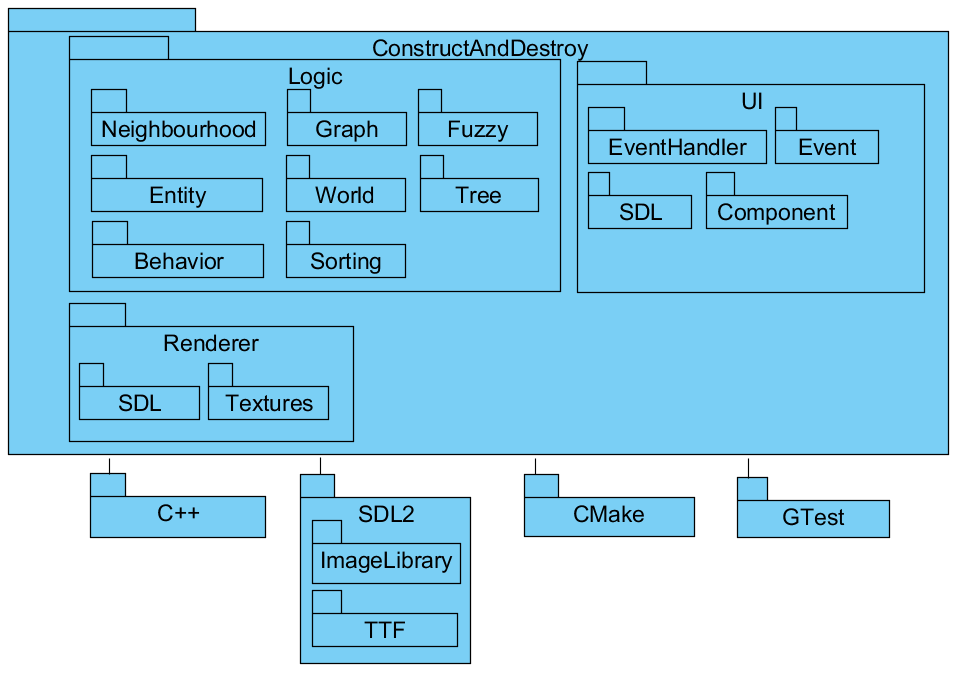
\includegraphics[scale=0.75]{res/high-level-overview.png}
    \caption{High level overview}\label{fig:system-overview}
\end{figure}

As shown in \cref{system-overview} the game has no dependency on databases or other servers and services. The game has three high level components: Logic, UI and Renderer. We have chosen this structure because of the Separation of Concern principle. All features of the game can be found in these components. The game is written in C++ and CMake is used for compilation. The unit tests are ran with GMake.
\newpage

\section{Steering}
Firstly, we're going to give some information about the base steering behaviour
 class. This class is an abstract class of which the other behaviours 
 inherit from. It has two methods, one for setting the targets and another for 
 calculating the produced force.
 \\
 Furthermore, we've applied the Strategy Pattern. We've done this because the 
 different steering behaviours don't differ much from eachother, except for 
 the actual force calculation. \cite{strategy-pattern}

~ \\
The base BehaviourStrategy class with the different implementations can be 
seen in the appendix at \cref{fig:behaviourstrategy}.

\subsection{Seek}
\label{sec:seek-behaviour}
The actual implementation for the seek strategy is actually quite short. The 
SeekStrategy class only uses the SeekStrategy::calculate\_force() method 
provided by the base BehaviourStrategy class.

The SeekStrategy generates an attractive force towards the target. It then 
scales the produces vector by an entity's max speed and subtracts the current 
velocity. \cite[pg. 91]{buckland}

The whole calculation can be represented by: \\
\large 
$$ force = \uvec{h} m - v $$
\normalsize

Where the unit vector $ \uvec{h} $ is the normalized heading (target position - 
our position), $ m $ is our maximum speed and v is our velocity.



\subsection{Flee}
In contrast to the previous behaviours, the FleeBehaviour creates a repulsive 
force which sends the entity away from the target. It looks a lot like the 
seek behaviour except that we check if the distance between us and the target 
exceeds a certain 'panic distance'. If it does, the resulting force equals 
$ \{0, 0, 0\} $. 

The actual force gets calculated by the following equation:
\large
$$ force = \uvec{h} m - v $$
\normalsize

Where $ \uvec{h} $ is our normalized heading vector which points away from 
our target (our position - target position).

As you can see, the FleeBehaviour is actually the opposite of our 
SeekBehaviour. \cite[pg. 92]{buckland}


\subsection{Arrive}
The arrive strategy looks a lot like the seek strategy, except that the 
closer we get to our target position the more we get slowed down
\cite[pg. 93]{buckland}. It uses the relation between speed and distance to 
scale our desired velocity. The ArriveStrategy class, like the SeekStrategy 
class, only uses the ArriveStrategy::calculate\_force() method.

The calculation can be represented as:
\large
$$ force = h \cdot (\frac{speed}{distance}) - v $$
\normalsize

Where $ h $ is our heading, $ v $ is our velocity and speed is:
\large
$$ speed = \min (\frac{distance}{deceleration}, max\_speed) $$
\normalsize

The deceleration variable is a constant which can be tweaked to make entities 
slow down more if needed.

If the distance variable is equal to zero, the vector returned by this method 
will just equal $ \{0, 0, 0\} $.


\subsection{Wander}
\label{sec:wander}
The wander force is a force which sends the entity into a random direction, 
based on it's wander\_angle variable. \\
The WanderStrategy projects a circle in front of an entity. The distance 
between this circle and the entity depends on the entity's current velocity. 
It is then normalized and scaled by a distance constant. So in other words; 
you can look at the circle's distance as our heading vector $ \uvec{h} $ on 
which a random (small) change gets applied \cite[pg. 96]{buckland}. 

To calculate the amount of displacement we create a vector $ v = \{ 0, -1\} $
 and scale it by the radius of our projected circle. Then we apply the current 
 wander\_angle variable with the following equation:

 \large
 $$ v = \{ \cos{(\angle wander)} \cdot |v|, \sin{(\angle wander)} \cdot |v| \} $$
 \normalsize

 The wander\_angle variable then gets incremented by another small random 
 number to be used in the next force calculation.

 The actual resulting wandering force is given by:

 \large
 $$ force = \uvec{h} + v $$
 \normalsize


\subsection{Obstacle Avoidance}
With the ObstacleAvoidanceBehaviour class, we try to steer away from the 
first target that enters our avoidance range.\cite[pg. 99]{buckland} 
\\
If there are no targets, the resulting force equals $ \{0, 0, 0\} $.

If there is a target, the resulting force is a normalized heading vector:
\large
$$ force = \uvec{h} $$
\normalsize

Where: 
\large
$$ h = (position + v) - target $$
\normalsize


\subsection{Explore}
\label{sec:explore}
The explore strategy checks if the entity has already explored the map, 
if it did, it already knows the positions of desired objects and can plan a 
path towards one of them. \\
If it did not already explore the map, it generates a path around the map 
which the entity needs to traverse. \\
The path consists of edges of a graph. The way this path gets calculated is 
by creating the longest path through the graph. This way we know that the 
entity will explore the whole map. \\
Lastly, the ExploreBehaviour uses the same calculation as the SeekBehaviour 
(\cref{sec:seek-behaviour}) for the produced force. It basically just moves to 
the next node in it's path.




\newpage

\section{Selection} In this chapter we will explain how our selection system
works. We will show which classes are involved and how the methods are chained
using UML-diagrams. 

\subsection{User interface} First off, how does the selecting feature works.
You can select a unit by clicking on it using the left mouse button. You can
select multiple by holding the left mouse button and dragging, while dragging a
rectangle is drawn. This rectangle represents the selecting area. When you
release the left mouse button every unit in the selecting area, the red
rectangle, will be selected. A selected unit is recognizable by the red line
around it.

\subsection{Selection process} First we made a handler that handles mouse input
for a panel that represents the world in the user interface. This is the
MouseHandler class, it derives from the SDL\_MouseEventSlot class which derives
from the Slot class. The SDL library provides us with low level access to the
mouse input on the window.  The header file of the MouseHandler can be found 
at \cref{lst:mousehandlerheader}.

\begin{lstlisting}[caption={Mouse handler header file.},
label={lst:mousehandlerheader}]
class MouseHandlerWorld : public SDL_MouseEventSlot {
private: 
    int start_drag_x; 
    int start_drag_y;
    void handle_up(sdl_mouse_event_data data); 
    void handle_down(sdl_mouse_event_data data); 
    void handle(sdl_mouse_event_data);
    void handle_motion(sdl_mouse_event_data);
    void handle_left_button(const vec2 &); 
    void handle_right_button(sdl_mouse_event_data &, const vec2 &);

public: 
    MouseHandlerWorld(); 
    ~MouseHandlerWorld(); 
    void on(sdl_mouse_event_data d) override; 
}; 
\end{lstlisting}

The class has a lot of private methods that handle the different types of mouse
events. It has one method that has been overridden from the base class, which
is the on-method. The on-method is where user inputs comes in. In this method
the input is separated into two groups and will be handled further by other
methods. To make it clear how this works an explanatory activity diagram can be
found at \cref{fig:activitymousehandler} in the appendix to illustrate the
process. 

After the on-method has determined whether the incoming data is a motion event
or button it will be handled further by other methods. We will start with the
motion input.

Motion input is handled by the handle\_motion method. Motion is only
important for us when the user is dragging. This means the user is holding the
left mouse button down while moving the mouse. When the user is dragging we set
the position the mouse has moved to and let the UI component know that the user
is dragging by setting a variable dragging to true. The UI component has two
methods called draw\_selection\_rectangle and render. Whenever the render
method is called and the variable dragging is true it will call the
draw\_selection\_rectangle with the positions set by the last call to the 
handle motion method.

Button input is handled a bit differently since we first need to determine what
kind of event it is and from which button. If the event comes from the right
button, it is an event that will control units. Since that has nothing to do
with this topic we will leave it there and explain it in a different chapter. 

If, however, the event does come from the left button it is to select units. 
When the left button is pressed down we get the position of the cursor. 
This will be the starting position of the selection rectangle. After a button 
down event from the left button, a button up event will inevitably be fired 
from the button. This event means a few things. First off all the user has 
stopped dragging, because we stated earlier that the user is dragging when he's 
holding down the left button. So we set the dragging variable to false. Also we 
reset the positions to be ready for a next drag event. After resetting the 
variables, we call the handle\_up method. This determines whether the event 
was a drag or a click of the left mouse button. A click is when you press and 
release the mouse in the same position or at maximum 10 pixels away from the 
original position. We have implemented it this way so it is easier to click 
moving targets. The handle\_left\_button\_click is called and it selects the 
target on the clicking position, unless there is no target in range.

When you release the left mouse button more than 10 pixels away from the origin
point you are dragging the mouse. The position of the release of the button and
the position of the press will passed to the select\_units\_in\_rectangle
method. The method first calculates the right, left, upper and bottom offsets 
for the rectangle. After this all units inside will be selected by checking 
which of the units that belong to the player are positioned inside the 
rectangle. At \cref{fig:selectiondrag} you can find a picture of a few 
units that are selected by the select\_units\_in\_rectangle function and you 
can also see the red rectangle that has been used to select them. 

\begin{figure}[H] 
    \centering
    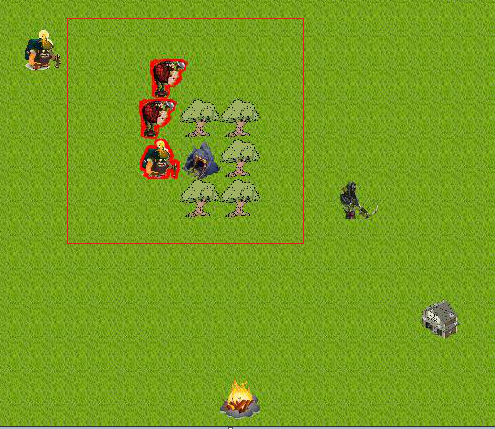
\includegraphics[scale=1.0]{res/SelectionRectangle.png} 
    \caption{Selection by dragging the mouse.}\label{fig:selectiondrag}
\end{figure} 

\newpage

\section{Graph} 
The graph is generated when the game/map is loaded. We’ve decided that our 
graph is a grid-like graph. We start off with generating the nodes, after that 
we generate adjacency edges. A node can have a maximum of 8 edges. When a 
static object is placed we remove edges from the node(s) on which the object 
is placed. We also remove the edges that lead to the node(s) on which the 
object is placed.

There is also a GraphManager which is a Singleton class to avoid making 
multiple graphs. It's also easy to access the graph in different parts of the 
code due to the GraphManager. 

\begin{figure}[H] 
    \centering 
    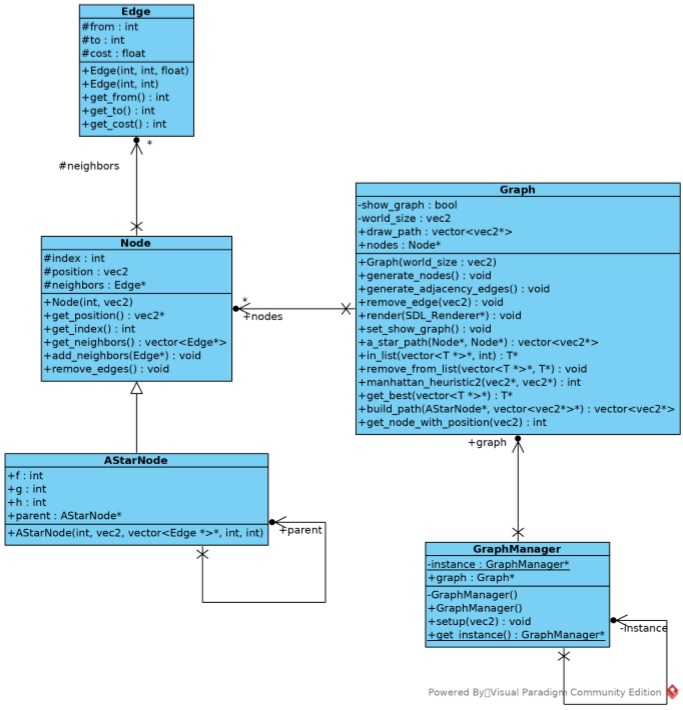
\includegraphics[scale=0.75]{res/graph.jpg}
    \caption{Class diagram for the Graph.}\label{fig:blue-line} 
\end{figure}

\newpage

\subsection{Path Planning}

\begin{tabularx}{\textwidth}{|X|X|}
\hline
\rowcolor{lightgray}\textcolor{white}{\textbf{Test scenario}} &
\textcolor{white}{\textbf{Desired result}}       
\\\hline
An entity plans a new path. &
Entity should plan the most efficient path and must avoid obstacles like buildings.
\\\hline
\rowcolor{lightgray}\textcolor{white}{\textbf{Comments/suggestions}} & 
\textcolor{white}{\textbf{Passed}}
\\\hline
 & \cellcolor{green}                       
\\\hline
\rowcolor{lightgray}\textcolor{white}{\textbf{Tester}} & 
\textcolor{white}{\textbf{Date}}               
\\\hline
Sander Bouwman & May 7, 2017                               		 
\\\hline
\end{tabularx}

\begin{tabularx}{\textwidth}{|X|X|}
\hline
\rowcolor{lightgray}\textcolor{white}{\textbf{Test scenario}} &
\textcolor{white}{\textbf{Desired result}}       
\\\hline
An entity plans a new path to an obstructed area. &
Entity shouldn't do anything because the area can't be reached.
\\\hline
\rowcolor{lightgray}\textcolor{white}{\textbf{Comments/suggestions}} & 
\textcolor{white}{\textbf{Passed}}
\\\hline
 & \cellcolor{green}                       
\\\hline
\rowcolor{lightgray}\textcolor{white}{\textbf{Tester}} & 
\textcolor{white}{\textbf{Date}}               
\\\hline
Sander Bouwman & May 7, 2017                               		 
\\\hline
\end{tabularx}
\newpage

\section{Behaviour}
\label{sec:behaviour}
We've chosen to use the goal driven behavior approach, because entities need to complete different actions to complete a goal. E.g., for a lumberjack to collect wood it needs to plan a path to the resource, then it needs to follow the path, once arrived it should start gathering, etc. Goal driven behavior provides a solid solution for these types of actions. Goals can be very large with loads off sub goals or actions, or they can be very small, this makes goal driven behavior easier extendable compared to state driven behavior for example. Since a goal can consist of multiple smaller goals, the Composite Pattern is a good solution to this problem. You can have small goals such as 'TraverseEdge' and also bigger goals like 'Work' and still treat them the same way. \cite{composite-pattern}

We created a single base class called Goal, which is a template class so that we can reuse it for different entity types. This class, together with the AtomicGoal and CompositeGoal classes, are shown in \cref{fig:goal}. Besides the Goal<T> class, we created two classes that inherit from it, the AtomicGoal and GoalComposite classes. The GoalComposite class contains a deque data structure that contains its subgoals. As you can see in \cref{fig:goal}, the GoalComposite<T> class also contains a couple of extra methods to add, remove, process and remove subgoals.

\subsection{Composite goals}
We created a couple of Composite goals for moving entities which we describe below. There is a class diagram \cref{fig:goalcomposite-inherit} in the appendix that illustrates the structure. This diagram doesn't show all composite goals, however it should give an impressions how we implemented this. 

\subsubsection{Think}
The Think goal is a goal that never gets removed. This goal is needed 
to determine an entity's next goal and activates that goal. It does so by 
calling the goals evaluator class, which returns a desirability value. The 
goal with the highest desirability gets chosen as the next goal. Desirability’s can be influenced by a variant of factors. E.g., how far away is the entity from an hostile entity. When there is an hostile enemy close it might not want to gather resources. Evaluators are a great way to create AI. Instead of using these evaluators we might use fuzzy logic. With fuzzy logic the actions of the entity should even feel more natural. 

\subsubsection{Follow Path}
\label{sec:followpath}
This goal traverses a path by adding the TraverseEdgeGoal class to its 
subgoals. This way a path consists of multiple instances of TraverseEdgeGoals
(\cref{sec:traverseedge}) which can be paused if the entity needs to do 
something else first, i.e. fleeing or resting. Once there are no more edges 
to traverse, this goal will be completed and removed from the entity's 
subgoals.

\subsubsection{Work}
This goal makes the entity go to the nearest resource to work. It first plans 
a path (\cref{sec:planpath}) to the nearest resource and then it follows that 
path (\cref{sec:followpath}). Once it arrives on the resource's location it 
starts to gather the resource (\cref{sec:gatherresource}). Once it's done 
gathering it plans another path, this time to the closest warehouse/depot. It follows 
this path and after it arrives it drops its resources 
(\cref{sec:dropresources}). Once all these goals are completed the work goal is completed as well.



\subsection{Atomic goals}
Besides Composite goals, we also have Atomic goals. You can compare Atomic 
goals with leaf nodes of a tree structure. Atomic goals are the actual actions
 that an entity needs to do. As shown in \cref{fig:atomicgoal-inherit}, an atomic 
 goal has no subgoals. Calling the AtomicGoal::add\_subgoal() method results in an 
 exception.
 
 \begin{figure}[!htb]
    \centering
    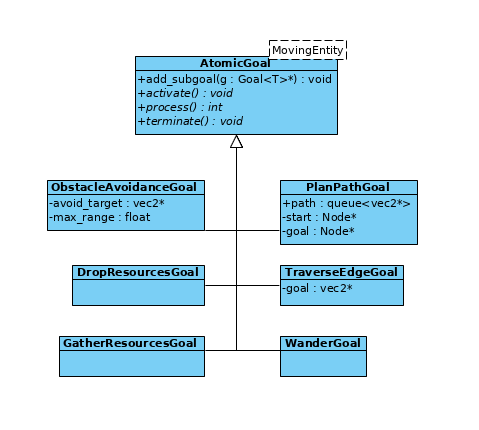
\includegraphics{res/AtomicGoal-Inherit.jpg}
    \caption{AtomicGoal Inheritance.}\label{fig:atomicgoal-inherit}
\end{figure}

\subsubsection{Wander}
The wandering goal is another goal that never gets removed, just like the 
think goal. An entity always needs to wander around if it has absolutely 
nothing to do. The only thing this goal does is activate the wander steering 
behaviour (\cref{sec:wander}).

\subsubsection{Obstacle Avoidance}
The obstacle avoidance goal activates the obstacle avoidance steering 
behaviour. When this goal is activated, it adds the steering behaviour to the 
entity's behaviours. Once the distance to the target that it needs to avoid 
is big enough, the goal is completed and the steering behaviour also gets 
removed from the entity.

\subsubsection{Drop Resources}
\label{sec:dropresources}
Once an entity has gathered enough resources, it needs to drop them at a 
warehouse/depot. This goal simply removes the resources the entity gathered and adds them to the resources of the player. When it dropped all of it's resources at the warehouse, the goal is completed.

\subsubsection{Gather Resource}
\label{sec:gatherresource}
This goal calls the Gather() method from a resource entity. This method extracts resources from the resource entity and adds it to the entity that is gathering the resource. Once the resource entity has been depleted or the maximum carrying capacity of the gathering entity has been reached this goal will be completed.

\subsubsection{Plan Path}
\label{sec:planpath}
The plan path goal plans a path using the A* algorithm, using the Manhattan 
heuristic (\cref{sec:pathplanning}). Once the path has been generated, it gets set as the active path 
for the given entity. This is the only task it needs to complete before 
getting removed from the containing goal.

\subsubsection{Traverse Edge}
\label{sec:traverseedge}
This goal uses the Seek behaviour explained in \cref{sec:seek-behaviour}. Once 
this class gets instantiated it adds an instance of SeekStrategy to the 
entity's behaviour. The only thing it needs to do while processing, is 
to check whether the entity has this behaviour, and if so if it's close 
enough to the next node on the graph. If it's close enough, the goal has been 
completed.


\newpage


\newpage

\section{User Interface}
\label{sec:ui}

Since we've chosen to use SDL2 as our rendering library, and SDL2 is just a 
microframework used for rendering to a window; we had to create our own GUI 
library. This means that we had to create a way to create and place GUI 
components like panels, buttons and text. This chapter will go in depth on 
how we created our own GUI library and how to use it.

\subsection{Templated UIComponent}
While creating the GUI library, we've used a lot of templating. This was done 
so that we can reuse our templated GUI classes if and when we decide to 
switch to OpenGL. The lowest level GUI class is called the UIComponent, 
which has a couple of template parameters for which rendering engine we're 
using,  the type of data its rendering object (see \cref{sec:rendering-ui} for 
an explanation about how the UIComponents get rendered.) contains, what kind 
of data it returns when rendering and the type of data for its mouse callback 
object (which will be explained in \cref{sec:eventhandling}).

The UIComponent class can be seen in \cref{fig:uicomponent}.

\begin{figure}[H]
\centering
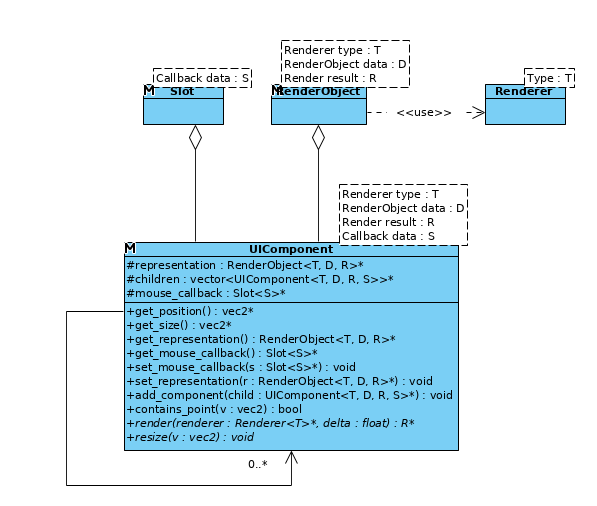
\includegraphics[scale=0.55]{res/ui/uicomponent.png}
\caption{UIComponent class.}\label{fig:uicomponent}
\end{figure}


\subsection{SDL2 GUI implementation}
\label{sec:sdl2gui}

Since we're using SDL2, we've made an implementation of the UIComponent class
 with the following template arguments:
\begin{itemize}
\item T = SDL\_Renderer (Rendering engine used by SDL2)
\item D = sdl\_data (a data structure)
\item R = SDL\_Texture (SDL2's texture structure)
\item S = sdl\_mouse\_event\_data (data used by the mouse callback object)
\end{itemize}

You can also create custom SDL\_UIComponent by inheriting from the 
SDL\_UIComponent class as shown in \cref{fig:sdluicomponent-inherit}. You can 
also use a custom struct that inherits from sdl\_data if your class' 
rendering object uses a different data type. For example, the SDLButton 
rendering object uses a struct that has been derived from the sdl\_data 
struct, which can be seen in \cref{lst:sdlbuttondata}.

\begin{figure}[!htb]
\centering
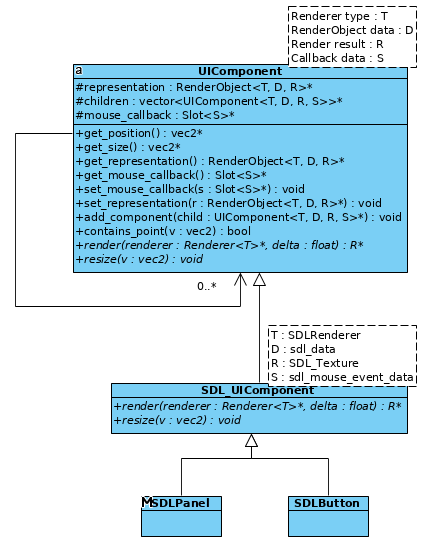
\includegraphics[scale=0.75]{res/ui/sdluicomponent-inherit.png}
\caption{SDL\_UIComponent class inheritance.}\label{fig:sdluicomponent-inherit}
\end{figure}



\newpage

\section{Rendering}
\label{sec:rendering}

In conjuction with creating our own GUI library, we've also created objects 
that handle the rendering of entities and UIComponents. This class is called 
the RenderObject, which is also a templated class so that we can reuse it 
if and when we decide to switch over to OpenGL rendering.

The Rendering class and its derived classes can be seen in 
\cref{fig:renderobject-inherit}.

\begin{figure}[!htb]
\centering
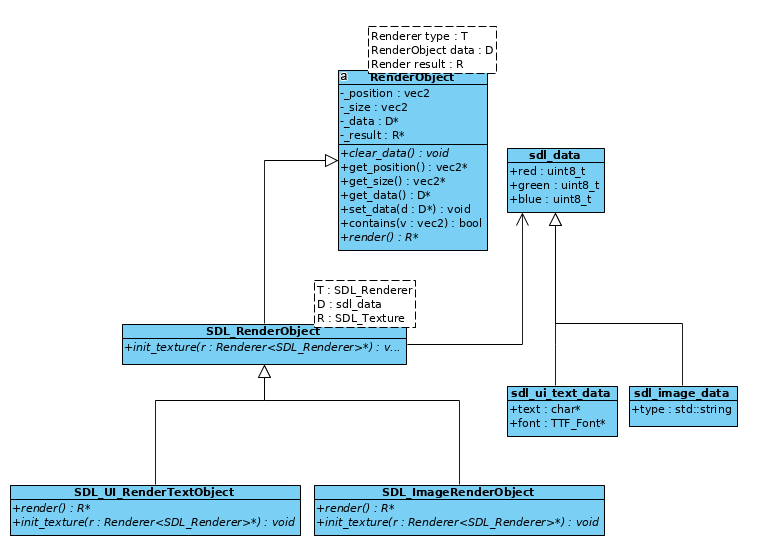
\includegraphics[scale=0.75]{res/renderobject-inherit.png}
\caption{RenderObject and derived classes}\label{fig:renderobject-inherit}
\end{figure}

\newpage
\subsection{Objects as a proxy}
\label{sec:rendering-proxy}

Objects that need to be rendered to the screen act as a proxy for the 
RenderObject. The only thing those objects need to do to be rendered can be 
seen in \cref{lst:rendering}. As you can see, the objects only need to return 
the result of its own RenderObject. Objects that need custom rendering logic 
can have a rendering object that derives from the SDL\_RenderObject class seen 
in \cref{fig:renderobject-inherit}.
\\
\begin{lstlisting}[caption={Rendering proxy.},label={lst:rendering}]
void BaseEntity::render(SDLRenderer *renderer) {
    return representation->render(renderer);
}
\end{lstlisting}

When a RenderObject renders itself, it sends the texture it created to the 
SDLRenderer class to draw it on a back buffer. After the rendering loop is 
completed, the back buffer is drawn to the screen using the 
\lstinline{renderer->draw_to_back_buffer(SDL_Texture *, SDL_Rect *)} 
method shown in \cref{lst:drawtobackbuffer}.
\\

\begin{lstlisting}[caption={Drawing to the back buffer.},
label={lst:drawtobackbuffer}]
void SDLRenderer::draw_to_back_buffer(SDL_Texture *t, SDL_Rect *r) {
    SDL_SetRenderTarget(engine, _back_buffer);
    // Blend the textures
    SDL_SetTextureBlendMode(_back_buffer, SDL_BLENDMODE_BLEND);
    SDL_SetTextureBlendMode(t, SDL_BLENDMODE_BLEND);
    if (SDL_RenderCopy(engine, t, NULL, r) < 0) {
        std::cerr << SDL_GetError() << std::endl;
    }
    SDL_SetRenderTarget(engine, NULL);
}
\end{lstlisting}

\subsection{UIComponent Rendering}
\label{sec:rendering-ui}

The uicomponents need a way of rendering their child components after 
rendering themselves. You can think of the relation between child components 
and their parent as a tree in which we first render the parent and then its 
children. The code for rendering a component and its children can be 
seen in \cref{lst:uicomponent-rendering}.
\\
\begin{lstlisting}[caption={UIComponent rendering.},
label={lst:uicomponent-rendering}]
void SDL_UIComponent::render(SDLRenderer *renderer, float delta) {
    representation->render(renderer);

    for (int i = 0; i < this->children.size(); i++) {
        children[i]->render(renderer, delta);
    }
}
\end{lstlisting}


\newpage

\subsection{Camera}

\begin{tabularx}{\textwidth}{|X|X|}
\hline
\rowcolor{lightgray}\textcolor{white}{\textbf{Test scenario}} &
\textcolor{white}{\textbf{Desired result}}       
\\\hline
Mouse cursor is not near an edge of the window. &
The camera does not move.         
\\\hline
\rowcolor{lightgray}\textcolor{white}{\textbf{Comments/suggestions}} & 
\textcolor{white}{\textbf{Passed}}
\\\hline
Null test & \cellcolor{green}                       
\\\hline
\rowcolor{lightgray}\textcolor{white}{\textbf{Tester}} & 
\textcolor{white}{\textbf{Date}}               
\\\hline
Robin Koning & June, 6, 2017                               		 
\\\hline
\end{tabularx}

\begin{tabularx}{\textwidth}{|X|X|}
\hline
\rowcolor{lightgray}\textcolor{white}{\textbf{Test scenario}} &
\textcolor{white}{\textbf{Desired result}}       
\\\hline
Cursor is near the left edge. &
Camera moves in the negative X direction.         
\\\hline
\rowcolor{lightgray}\textcolor{white}{\textbf{Comments/suggestions}} & 
\textcolor{white}{\textbf{Passed}}
\\\hline
 & \cellcolor{green}                       
\\\hline
\rowcolor{lightgray}\textcolor{white}{\textbf{Tester}} & 
\textcolor{white}{\textbf{Date}}               
\\\hline
Robin Koning & June, 6, 2017                               		 
\\\hline
\end{tabularx}

\begin{tabularx}{\textwidth}{|X|X|}
\hline
\rowcolor{lightgray}\textcolor{white}{\textbf{Test scenario}} &
\textcolor{white}{\textbf{Desired result}}       
\\\hline
Cursor is near the top edge. &
Camera moves in the negative Y direction.         
\\\hline
\rowcolor{lightgray}\textcolor{white}{\textbf{Comments/suggestions}} & 
\textcolor{white}{\textbf{Passed}}
\\\hline
 & \cellcolor{green}                       
\\\hline
\rowcolor{lightgray}\textcolor{white}{\textbf{Tester}} & 
\textcolor{white}{\textbf{Date}}               
\\\hline
Robin Koning & June, 6, 2017                               		 
\\\hline
\end{tabularx}

\begin{tabularx}{\textwidth}{|X|X|}
\hline
\rowcolor{lightgray}\textcolor{white}{\textbf{Test scenario}} &
\textcolor{white}{\textbf{Desired result}}       
\\\hline
Cursor is near the right edge. &
Camera moves in the positive X direction.         
\\\hline
\rowcolor{lightgray}\textcolor{white}{\textbf{Comments/suggestions}} & 
\textcolor{white}{\textbf{Passed}}
\\\hline
 & \cellcolor{green}                       
\\\hline
\rowcolor{lightgray}\textcolor{white}{\textbf{Tester}} & 
\textcolor{white}{\textbf{Date}}               
\\\hline
Robin Koning & June, 6, 2017                               		 
\\\hline
\end{tabularx}

\begin{tabularx}{\textwidth}{|X|X|}
\hline
\rowcolor{lightgray}\textcolor{white}{\textbf{Test scenario}} &
\textcolor{white}{\textbf{Desired result}}       
\\\hline
Cursor is near the bottom edge. &
Camera moves in the positive Y direction.         
\\\hline
\rowcolor{lightgray}\textcolor{white}{\textbf{Comments/suggestions}} & 
\textcolor{white}{\textbf{Passed}}
\\\hline
 & \cellcolor{green}                       
\\\hline
\rowcolor{lightgray}\textcolor{white}{\textbf{Tester}} & 
\textcolor{white}{\textbf{Date}}               
\\\hline
Robin Koning & June, 6, 2017                               		 
\\\hline
\end{tabularx}

\begin{tabularx}{\textwidth}{|X|X|}
\hline
\rowcolor{lightgray}\textcolor{white}{\textbf{Test scenario}} &
\textcolor{white}{\textbf{Desired result}}       
\\\hline
Cursor is near the left edge and camera position is \{0,0\}. &
Camera does not move.         
\\\hline
\rowcolor{lightgray}\textcolor{white}{\textbf{Comments/suggestions}} & 
\textcolor{white}{\textbf{Passed}}
\\\hline
 & \cellcolor{green}                       
\\\hline
\rowcolor{lightgray}\textcolor{white}{\textbf{Tester}} & 
\textcolor{white}{\textbf{Date}}               
\\\hline
Robin Koning & June, 6, 2017                               		 
\\\hline
\end{tabularx}

\begin{tabularx}{\textwidth}{|X|X|}
\hline
\rowcolor{lightgray}\textcolor{white}{\textbf{Test scenario}} &
\textcolor{white}{\textbf{Desired result}}       
\\\hline
Cursor is near the top edge and camera position is \{0,0\}. &
Camera does not move.         
\\\hline
\rowcolor{lightgray}\textcolor{white}{\textbf{Comments/suggestions}} & 
\textcolor{white}{\textbf{Passed}}
\\\hline
 & \cellcolor{green}                       
\\\hline
\rowcolor{lightgray}\textcolor{white}{\textbf{Tester}} & 
\textcolor{white}{\textbf{Date}}               
\\\hline
Robin Koning & June, 6, 2017                               		 
\\\hline
\end{tabularx}

\begin{tabularx}{\textwidth}{|X|X|}
\hline
\rowcolor{lightgray}\textcolor{white}{\textbf{Test scenario}} &
\textcolor{white}{\textbf{Desired result}}       
\\\hline
Cursor is near the right edge and camera position is \{worldsize.x,0\}. &
Camera does not move.         
\\\hline
\rowcolor{lightgray}\textcolor{white}{\textbf{Comments/suggestions}} & 
\textcolor{white}{\textbf{Passed}}
\\\hline
 & \cellcolor{green}                       
\\\hline
\rowcolor{lightgray}\textcolor{white}{\textbf{Tester}} & 
\textcolor{white}{\textbf{Date}}               
\\\hline
Robin Koning & June, 6, 2017                               		 
\\\hline
\end{tabularx}

\begin{tabularx}{\textwidth}{|X|X|}
\hline
\rowcolor{lightgray}\textcolor{white}{\textbf{Test scenario}} &
\textcolor{white}{\textbf{Desired result}}       
\\\hline
Cursor is near the bottom edge and camera position is \{0,worldsize.y\}. &
Camera does not move.         
\\\hline
\rowcolor{lightgray}\textcolor{white}{\textbf{Comments/suggestions}} & 
\textcolor{white}{\textbf{Passed}}
\\\hline
 & \cellcolor{green}                       
\\\hline
\rowcolor{lightgray}\textcolor{white}{\textbf{Tester}} & 
\textcolor{white}{\textbf{Date}}               
\\\hline
Robin Koning & June, 6, 2017                               		 
\\\hline
\end{tabularx}

\begin{tabularx}{\textwidth}{|X|X|}
\hline
\rowcolor{lightgray}\textcolor{white}{\textbf{Test scenario}} &
\textcolor{white}{\textbf{Desired result}}       
\\\hline
Scrollwheel up. &
World and entities get scaled up.         
\\\hline
\rowcolor{lightgray}\textcolor{white}{\textbf{Comments/suggestions}} & 
\textcolor{white}{\textbf{Passed}}
\\\hline
The direction of scrolling might be flipped depending on system. & \cellcolor{green}                       
\\\hline
\rowcolor{lightgray}\textcolor{white}{\textbf{Tester}} & 
\textcolor{white}{\textbf{Date}}               
\\\hline
Robin Koning & June, 6, 2017                               		 
\\\hline
\end{tabularx}

\begin{tabularx}{\textwidth}{|X|X|}
\hline
\rowcolor{lightgray}\textcolor{white}{\textbf{Test scenario}} &
\textcolor{white}{\textbf{Desired result}}       
\\\hline
Scrollwheel down. &
World and entities get scaled down.         
\\\hline
\rowcolor{lightgray}\textcolor{white}{\textbf{Comments/suggestions}} & 
\textcolor{white}{\textbf{Passed}}
\\\hline
The direction of scrolling might be flipped depending on system. & \cellcolor{green}                       
\\\hline
\rowcolor{lightgray}\textcolor{white}{\textbf{Tester}} & 
\textcolor{white}{\textbf{Date}}               
\\\hline
Robin Koning & June, 6, 2017                               		 
\\\hline
\end{tabularx}

\newpage

\section{Event Handling}
\label{sec:eventhandling}

In this chapter we'll go in depth about how the event handling works and how 
to use and create event objects. We'll explain what slots are in 
\cref{sec:slots} and how to register a slow to the event dispatcher in 
\cref{sec:eventdispatch}.

\subsection{Slots}
\label{sec:slots}

As seen in \cref{fig:sdluicomponent-inherit}, a UIComponent also has a 
Slot<S> object. This object handles the mouse events for the component.
A class diagram showing the Slot class and derived classes are shown in 
\cref{fig:slot-inherit}.

\begin{figure}[!htb]
    \centering
    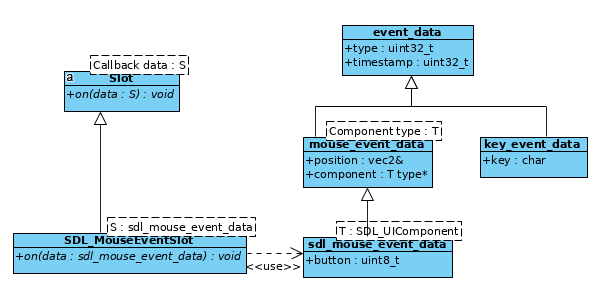
\includegraphics[scale=0.7]{res/events/slot.png}
    \caption{Slot and derived classes.}\label{fig:slot-inherit}
\end{figure}

\subsection{Event dispatching}
\label{sec:eventdispatch}
We've decided to create a system that handles the dispatching of events. This 
system looks a lot like an Observer Pattern. Instead of registering observers 
to a subject, we register slots and uicomponents to the event dispatcher.
This EventDispatcher class then decides in its dispatch method where to send 
the event to. We've done this so that when, for example, we move the mouse 
on the world panel, we don't call the other panel's callback function.
What the event dispatcher looks like and its relation with ui components and 
slots are shown in \cref{fig:eventdispatcher}.

\begin{figure}[H]
\centering
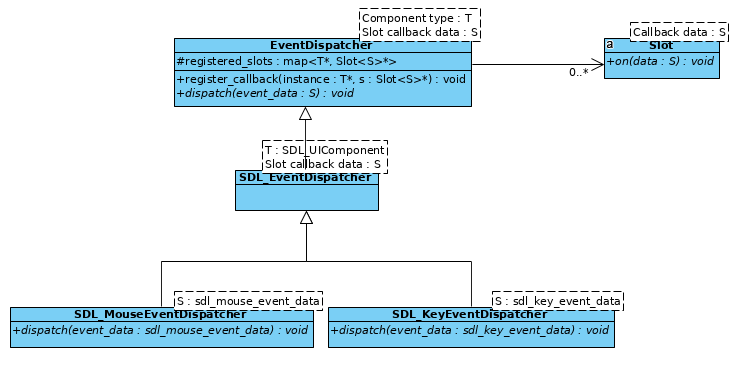
\includegraphics[scale=0.6]{res/events/eventdispatch.png}
\caption{The EventDispatcher and derived classes}\label{fig:eventdispatcher}
\end{figure}

\subsubsection{Calling the right panel's slot.}
\label{sec:eventdispatcher-dispatch}
As we've mentioned before, when we send an event, we don't want to call each 
panel's callback slot. We needed to create some logic for deciding where to 
send the event, which can be seen in \cref{lst:sdleventdispatch}.
\\

\begin{lstlisting}[caption={SDL\_MouseEventDispatcher dispatch method.},
label={lst:sdleventdispatch}]
void SDL_MouseEventDispatcher::dispatch(sdl_mouse_event_data d) {
    SDL_UIComponent *best_component = nullptr;
    Slot<sdl_mouse_event_data> *best_slot = nullptr;
    for (std::map<SDL_UIComponent *, Slot<sdl_mouse_event_data> *>::iterator it = _registered_slots.begin();
         it != _registered_slots.end(); ++it) {
        SDL_UIComponent *current_component = (*it).first;
        float current_distance = current_component->get_position()->distance(d.position);
        if (current_component->contains_point(d.position) &&
            (!best_slot || current_distance < best_component->get_position()->distance(d.position))) {
            best_component = current_component;
            best_slot = (*it).second;
        }
    }
    if (best_slot) {
        d.component = best_component;
        best_slot->on(d);
    }
}
\end{lstlisting}


\newpage

\section{Selection} In this chapter we will explain how our selection system
works. We will show which classes are involved and how the methods are chained
using UML-diagrams. 

\subsection{User interface} First off, how does the selecting feature works.
You can select a unit by clicking on it using the left mouse button. You can
select multiple by holding the left mouse button and dragging, while dragging a
rectangle is drawn. This rectangle represents the selecting area. When you
release the left mouse button every unit in the selecting area, the red
rectangle, will be selected. A selected unit is recognizable by the red line
around it.

\subsection{Selection process} First we made a handler that handles mouse input
for a panel that represents the world in the user interface. This is the
MouseHandler class, it derives from the SDL\_MouseEventSlot class which derives
from the Slot class. The SDL library provides us with low level access to the
mouse input on the window.  The header file of the MouseHandler can be found 
at \cref{lst:mousehandlerheader}.

\begin{lstlisting}[caption={Mouse handler header file.},
label={lst:mousehandlerheader}]
class MouseHandlerWorld : public SDL_MouseEventSlot {
private: 
    int start_drag_x; 
    int start_drag_y;
    void handle_up(sdl_mouse_event_data data); 
    void handle_down(sdl_mouse_event_data data); 
    void handle(sdl_mouse_event_data);
    void handle_motion(sdl_mouse_event_data);
    void handle_left_button(const vec2 &); 
    void handle_right_button(sdl_mouse_event_data &, const vec2 &);

public: 
    MouseHandlerWorld(); 
    ~MouseHandlerWorld(); 
    void on(sdl_mouse_event_data d) override; 
}; 
\end{lstlisting}

The class has a lot of private methods that handle the different types of mouse
events. It has one method that has been overridden from the base class, which
is the on-method. The on-method is where user inputs comes in. In this method
the input is separated into two groups and will be handled further by other
methods. To make it clear how this works an explanatory activity diagram can be
found at \cref{fig:activitymousehandler} in the appendix to illustrate the
process. 

After the on-method has determined whether the incoming data is a motion event
or button it will be handled further by other methods. We will start with the
motion input.

Motion input is handled by the handle\_motion method. Motion is only
important for us when the user is dragging. This means the user is holding the
left mouse button down while moving the mouse. When the user is dragging we set
the position the mouse has moved to and let the UI component know that the user
is dragging by setting a variable dragging to true. The UI component has two
methods called draw\_selection\_rectangle and render. Whenever the render
method is called and the variable dragging is true it will call the
draw\_selection\_rectangle with the positions set by the last call to the 
handle motion method.

Button input is handled a bit differently since we first need to determine what
kind of event it is and from which button. If the event comes from the right
button, it is an event that will control units. Since that has nothing to do
with this topic we will leave it there and explain it in a different chapter. 

If, however, the event does come from the left button it is to select units. 
When the left button is pressed down we get the position of the cursor. 
This will be the starting position of the selection rectangle. After a button 
down event from the left button, a button up event will inevitably be fired 
from the button. This event means a few things. First off all the user has 
stopped dragging, because we stated earlier that the user is dragging when he's 
holding down the left button. So we set the dragging variable to false. Also we 
reset the positions to be ready for a next drag event. After resetting the 
variables, we call the handle\_up method. This determines whether the event 
was a drag or a click of the left mouse button. A click is when you press and 
release the mouse in the same position or at maximum 10 pixels away from the 
original position. We have implemented it this way so it is easier to click 
moving targets. The handle\_left\_button\_click is called and it selects the 
target on the clicking position, unless there is no target in range.

When you release the left mouse button more than 10 pixels away from the origin
point you are dragging the mouse. The position of the release of the button and
the position of the press will passed to the select\_units\_in\_rectangle
method. The method first calculates the right, left, upper and bottom offsets 
for the rectangle. After this all units inside will be selected by checking 
which of the units that belong to the player are positioned inside the 
rectangle. At \cref{fig:selectiondrag} you can find a picture of a few 
units that are selected by the select\_units\_in\_rectangle function and you 
can also see the red rectangle that has been used to select them. 

\begin{figure}[H] 
    \centering
    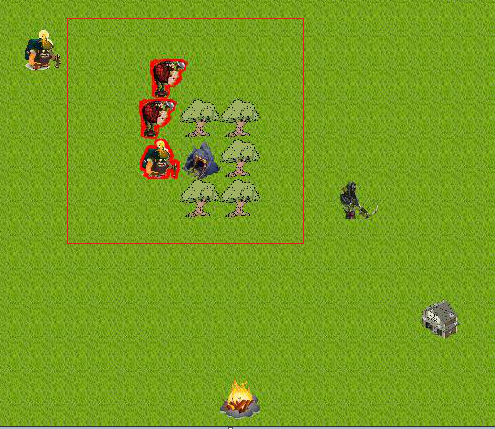
\includegraphics[scale=1.0]{res/SelectionRectangle.png} 
    \caption{Selection by dragging the mouse.}\label{fig:selectiondrag}
\end{figure} 

\newpage

\section{Controlling workers}

One of the things the player can do is order workers to do a specific task. This is done by selecting one or more workers followed by right clicking somewhere. For example, the player can right click on the ground, which will cause the selected workers to move there. The player can also order workers to gather resources such as wood.

Since the player can select any kind of worker and order it to do many different things, a design pattern was needed to ensure that the code remained readable and extensible. The strategy pattern was chosen because of the fact that it is very extensible. 

A class diagram of relevant classes can be found in \cref{fig:orderstrategies}. The basic idea is that there is one singleton class named MoveOrder with a orderMove function. This function can be used throughout the game to order one or more entities to do something at a certain vector. Based on what the player right clicked on an OrderStrategy is selected. This OrderStrategy takes care of the right click event, for example by ordering the selected entities to go to a certain location.

Down below, in \cref{fig:orderstrategy}, you can find the implementation of the strategy that handles the event where a user orders one or more entities to move to a piece of ground.

\begin{figure}[!htb]
    \centering
    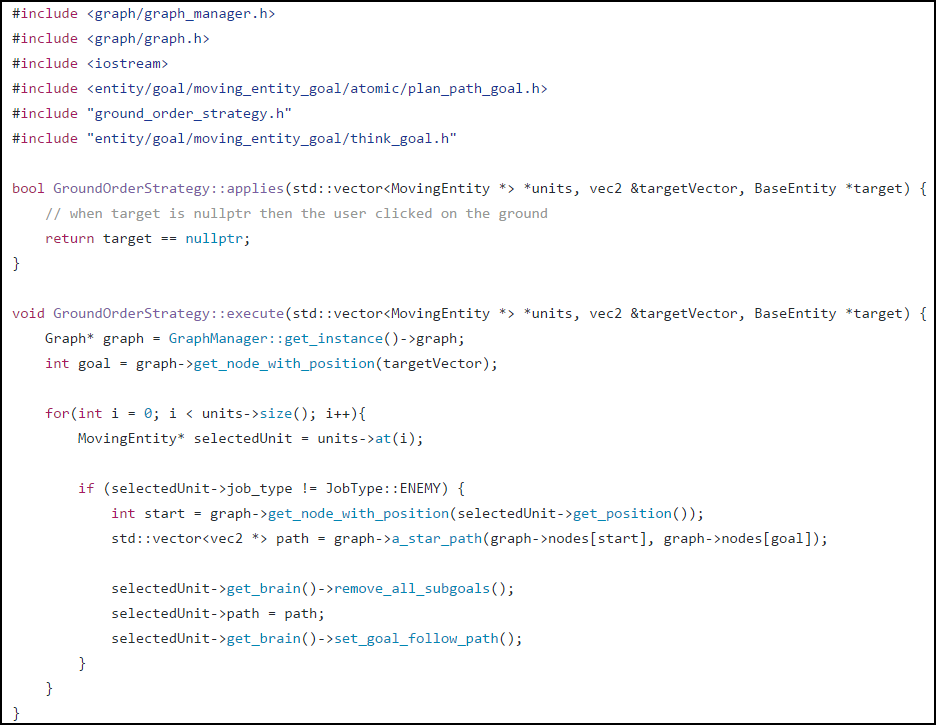
\includegraphics[angle=0,origin=c,scale=0.66]
    {images/order-strategy.PNG}
    \caption{Order strategy}\label{fig:orderstrategy}
\end{figure}


\newpage

\section{Adding buildings} 
\label{sec:addingbuildings} 
As a player you may want to add buildings to the world. In this section we 
will explain how a player can add buildings and how we have implemented this 
feature.

\subsection{Controls and feedback} 
Buildings can be spawned using the building panel (see 
\cref{fig:building-panel}). When the player clicks on the building that he/she 
wishes to spawn, or presses the key that belongs to the building
(displayed in the top left corner of the building in the building panel), a
slightly transparent texture of the building appears at the mouse position.
When the player hovers the mouse over another static entity, the texture gets a
red border. This will notify the player that the building cannot be placed at
that current mouse position. If the player decides not to place a building
after all, the action can be cancelled by pressing the escape key. More 
information about this subject can be found at \cref{AbortPlacingBuilding}. 
When the player is satisfied with the position to place the building on, it 
can be placed by clicking the left mouse button. 

\subsection{Building panel} 
The building panel, as displayed in \cref{fig:building-panel}, iterates over 
the buildings\_with\_textures enumeration, and for each entry it adds a 
UnitPanel to the Building Panel. UnitPanels are used for the EntityPanel (see 
\cref{fig:entity-panel}) as well as the Building Panel. These UnitPanels render an 
image, and contain objects of whatever it renders (buildings or entities). 
Unit panels are highlighted in \cref{fig:unit-panel} in the appendix.

A mouse handler (of which a diagram is shown in
\cref{fig:mousehandlerbuildingpanel}), or the key event handler takes care of
actually starting the process of positioning and placing a building. The
shortcut keys to start this process are located at the top left corner of the
unit panel, as shown in \cref{fig:building-shortcuts}.

\subsection{States} 
We are using the state pattern during positioning and placing buildings, 
because this pattern makes it easy to extend the behaviour of the player or 
entity, which can be different each state.\\ 
When a player clicks on a building in the building panel, the mouse handler 
will look at the player's current state. If the player is already in the
ChoosingBuildingPosition state, then the player wants to set the current mouse
position as the final position of the building, and the player's state will
change to the  PlacingBuilding state.\\ 
If the player is not in the ChoosingBuildingState state, the mouse  handler 
will call the choosing\_building\_position method, which belongs to the 
BuildingManager. The building manager is responsible for creating the 
building entity, together with the BuildingFactory.  When the entity is 
created, it will be added to the world so this object will be rendered.  
The BuildingManager will also set the positioning\_object variable of the 
player, so the player can keep track of the building it is positioning from 
now on. After all this is done, the state of the player will be changed to 
ChoosingBuildingPosition.  A state machine diagram explaining state 
transitions can be found in \cref{fig:statediagram-addingbuildings} and a 
class diagram with relevant methods, associations and variables can be found in
\cref{fig:classdiagram-addingbuildings}.

\begin{figure}[H] 
    \centering
    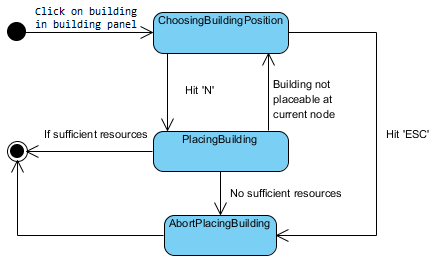
\includegraphics{res/adding-buildings/States-StateDiagram.png} 
    \caption{Adding buildings state diagram.}\label{fig:statediagram-addingbuildings} 
\end{figure}

\subsubsection{ChoosingBuildingPosition} 
At entering this state, the texture its opacity will be set to 70\%. We have 
chosen to do so, because this will make it clear which objects are already 
placed and which objects are not placed by the player yet.\\ During the 
execute method of this state the mouse position of the player will be tracked. 
If the mouse position has changed, the GraphManager will be consumed to get 
the nearest node in relation to the mouse position. If there is another static 
entity on that node, we want to inform the player by changing the entity's 
texture by adding a red border.

\subsubsection{PlacingBuilding} 
The PlacingBuilding state will be entered when the player clicks the left 
mouse button in the game world while it is in the ChoosingBuildingPosition 
state. This state only has logic in its enter method, because it needs to 
make one decision: can the building be positioned at this position or not.\\ 
If the building cannot be positioned at the node, the state will be changed 
back to ChoosingBuildingPosition, to give the user another chance to find a 
good spot for the building. If the building can be placed at the node and the 
player has enough resources to cover the costs for a building, the entity will 
be added to the building array of the player and to the building array of the 
BuildingManager. The costs of the building will be subtracted from the player 
its gathered resources. The opacity will also be set to 0\%. The 
positioning\_object variable kept by the player object will be cleared, just 
like the current state of the user.

\subsubsection{AbortPlacingBuilding} 
\label{AbortPlacingBuilding} 
This state will be entered when a player is in the ChoosingBuildingPosition 
state and it hits the 'ESC' key. It also will be entered after a player enters 
the PlacingBuilding state and it does not have enough resources to place the 
building. The method only has logic in the enter method and it calls the 
remove\_building() method from the BuildingFactory. 

\begin{figure}[H] 
    \centering
    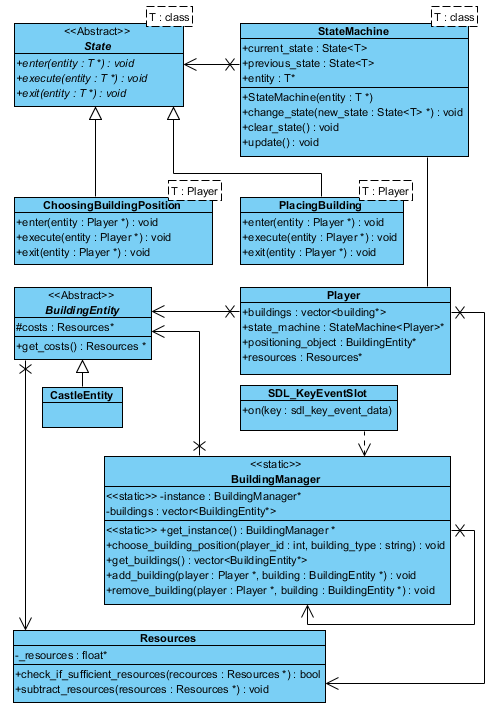
\includegraphics{res/adding-buildings/States-ClassDiagram.png} 
    \caption{Adding buildings class diagram.}\label{fig:classdiagram-addingbuildings} 
\end{figure}

\newpage

\section{Creating units}
In this chapter we will explain how creating units is implemented in the game. We will go through some of the code and show the design patterns we used.

\subsection{Entity Panel} \label{sec:EntityPanel}
A unit can be created in a building, in a castle for example. When the player selects a castle the building panel is replaced by a different panel which shows all units that can be spawned from the selected building. This can be seen in \cref{fig:entity-panel}, where the entity panel is the panel at the bottom of the screen. 

A player can order many entities, but they won't be spawned right away. Instead, they are queued. The number of entities in the build queue are displayed in a badge. Only one entity can be spawned at a given time. The color of the badge indicates whether an entity is being built and how close it is to actually spawning. 

All variations of the badge can be seen in \cref{fig:unit-panel-order-queue}. If there aren't any entities in the queue, then the badge is grey. If there are entities in the queue, but it isn't currently being built, then the badge is grey as well. When an entity is building, the badge has a red background at first which slowly changes to green over time, and is solid green just before the entity gets spawned.

The cost of spawning an entity can be seen below each entity itself in the panel. The cost will turn red if the player does not have sufficient resources to train the entity. 

If the player wants additional information about something the available entities in the panel the player can hover over the units image. This will trigger a description in the topleft corner giving a short explanation of what the entity does. E.g. for a Knight the description will say something like: "This unit will fight for the safety of you village" and for a lumberjack it will say: "This unit will gather wood."

In \cref{fig:unit-panel} all unit panels are highlighted. For each unit that can be spawned from the selected building, a unit panel is added to the entity panel at the bottom of the screen. A unit panel, as displayed in \cref{fig:unit-panel-class-diagram}, contains the EntityType that belongs to a unit panel which it uses to render the sprite that belongs to the EntityType.

In order to capture click events, and trigger the unit spawning process, a MouseHandlerEntityPanel is used. When the player clicks on an entity, the mouse handler takes care of spawning the unit and subtracing the resource cost. The entity will only be ordered if the player has enough resources to pay for the unit, as shown below.

Another way to spawn a unit is to press the shortcut key. This shortcut key is shown in the top left badge of the unit panel, as you can see in  \cref{fig:entity-shortcuts}.

\begin{lstlisting}
 if (p->resources->check_if_sufficient_resources(spawnable_entity->get_cost())) {
    // tell the building to spawn the selected entity type
    building->order_unit(spawnable_entity->get_entity_type());
    
    p->resources->subtract_resources(spawnable_entity->get_cost());
}
\end{lstlisting}

\subsection{Ordering units}
When a user orders a unit from a building we will look at the order time of the castle which represents the time the castle needs to create the unit. This time can be seen as time that is needed to train the unit and make it ready to participate in your world to give it a more realistic feeling than spawning the unit immediately on the screen. 

When the player orders a unit. The following method is called:

\begin{lstlisting}
void CastleEntity::order_unit(MovingEntityType moving_entity_type) {
    this->orders.push_back(moving_entity_type);
}
\end{lstlisting}

We add the type of the unit to a vector called orders. In which the orders placed by the player on that building are saved. The order is pushed to the back of the vector so that the array somewhat resembles a queue. A enum member of the enum MovingEntityType is used to determine what kind of unit needs to be created. After the completion of this method a unit is successfully ordered and waits for time to pass to be created.

\subsection{Handling the orders}
To handle orders placed in the building we use the update method. The update method is called every game-update so it is perfect to calculate time and decide if anything needs to be done with the orders. Below you can see the code of the update method:

%-- Do not worry about the code listings being half on two different pages. This will be fixed when Jeroen is done. 

\begin{lstlisting}
void CastleEntity::update(float d) {
    if(!this->orders.empty()){
        delta_time += d;
        if(delta_time >= order_time){


            this->order_unit_from_factory(_player, spawn, orders.front());

            //remove first from orders.
            orders.erase(orders.begin());
 
            //reset order time.
            delta_time = 0;
        }
    };
}
\end{lstlisting}

First we check if order is not empty. If that is the case, we update the delta\_time. This is so we know the time that has passed since the an order was placed. Then we check if the order\_time, the time it takes to create a unit, has been surpassed by the time that has passed since the order was placed. If that is the case we handle off the order of the unit by calling the method order\_unit\_from\_factory which we will explain below. After ordering from the factory, we take out the order from the orders vector since the order has been handled. And we also reset the delta\_time to zero so we can handle the next order after the same order\_time.

\subsection{MovingEntity Factory}
The order\_unit\_from\_factory method calls the MovingEntityManager's method add\_unit. As parameters it provides:

\begin{itemize}  
\item A Player*, the player for which the unit has to be created.
\item A vec2 Position, the X and Y coordinates where the unit should be spawned.
\item A MovingEntityType, type of the unit(FE: Lumberjack, Miner, Knight and more...)
\end{itemize}
The MovingEntityManager handles any interaction with the factory. And uses the parameters to call the factory and create the unit. We have implemented the structure of this code like a factory pattern as can be seen in the following class diagram below. The class diagram found at \cref{fig:movingentityfactory} focusses on the factory and the classes that use and so only the really important classes are completely shown with all it's methods and attributes.  

After the MovingEntityManager has completed an order from the factory the unit will spawn in the given location. This process will repeat until all orders have been handled.





\newpage

\subsection{Unit information panel}

\begin{tabularx}{\textwidth}{|X|X|}
\hline
\rowcolor{lightgray}\textcolor{white}{\textbf{Test scenario}} &
\textcolor{white}{\textbf{Desired result}}       
\\\hline
Single entity information &
When a single entity is selected, a panel in the bottom right corner appears containing information about the selected entity
\\\hline
\rowcolor{lightgray}\textcolor{white}{\textbf{Comments/suggestions}} & 
\textcolor{white}{\textbf{Passed}}
\\\hline
 & \cellcolor{green}                       
\\\hline
\rowcolor{lightgray}\textcolor{white}{\textbf{Tester}} & 
\textcolor{white}{\textbf{Date}}               
\\\hline
Jeroen Vinke & June 7, 2017                               		 
\\\hline
\end{tabularx}

\begin{tabularx}{\textwidth}{|X|X|}
\hline
\rowcolor{lightgray}\textcolor{white}{\textbf{Test scenario}} &
\textcolor{white}{\textbf{Desired result}}       
\\\hline
Building information &
When a building is selected, a panel in the bottom right corner appears containing information about the selected building
\\\hline
\rowcolor{lightgray}\textcolor{white}{\textbf{Comments/suggestions}} & 
\textcolor{white}{\textbf{Passed}}
\\\hline
 & \cellcolor{green}                       
\\\hline
\rowcolor{lightgray}\textcolor{white}{\textbf{Tester}} & 
\textcolor{white}{\textbf{Date}}               
\\\hline
Jeroen Vinke & June 7, 2017                               		 
\\\hline
\end{tabularx}

\begin{tabularx}{\textwidth}{|X|X|}
\hline
\rowcolor{lightgray}\textcolor{white}{\textbf{Test scenario}} &
\textcolor{white}{\textbf{Desired result}}       
\\\hline
Multiple entity information &
When multiple entities are selected, a panel in the bottom right corner appears containing images of the entities that are selected
\\\hline
\rowcolor{lightgray}\textcolor{white}{\textbf{Comments/suggestions}} & 
\textcolor{white}{\textbf{Passed}}
\\\hline
 & \cellcolor{green}                       
\\\hline
\rowcolor{lightgray}\textcolor{white}{\textbf{Tester}} & 
\textcolor{white}{\textbf{Date}}               
\\\hline
Jeroen Vinke & June 7, 2017                               		 
\\\hline
\end{tabularx}
\newpage

\section{Waves}
\label{sec:waves}

In this chapter we'll explain how the wave system is implemented in our game. 
We will show some diagrams concerning the wave system and its information 
panel.

\subsection{Implementation}
\label{sec:wave-implementation}

To implement a wave system, we created a class called Wave which handles the 
spawning of new units and incrementing the wave counter and stat modifier.
This class and its relations are shown in \cref{fig:wave}.

\begin{figure}[H]
    \centering
    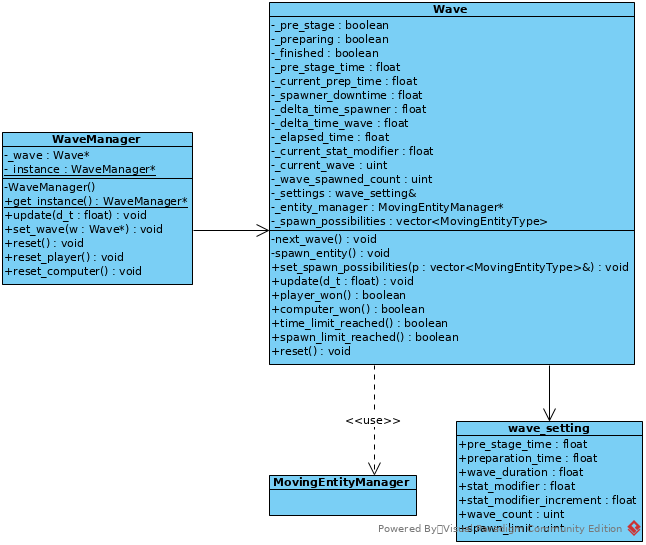
\includegraphics[scale=0.6]{res/wave.png}
    \caption{Wave class and relations.}\label{fig:wave}
\end{figure}

Every update cycle, the update method of wave gets called. In this update 
method we check whether the wave is in a preparation state. If it is we 
simply decrement the preparation time variable with the delta time passed to 
the update method. If we're in a spawning state, we check whether we've 
already spawned the maximum amount of entities for this wave. If not, we spawn 
an entity, increment the entity counter and decrement the spawning timer.

Once we've checked if we need to spawn an entity, we need to check if we 
reached the next wave. If so, we increment the wave counter and the stat 
modifier and we reset the amount of entities spawned in the wave so that we 
can spawn new entities this wave.

The code for this is shown in \cref{lst:wave-update}.
\\
\begin{lstlisting}[caption={Spawning entities and next wave.},
label={lst:wave-update}]
if(!_preparing) {
    _delta_time_wave += delta;
    _delta_time_spawner += delta;
    _elapsed_time += delta;
    if(!spawn_limit_reached()) {
        spawn_entity();
    } else if(spawn_limit_reached() && _current_wave < _settings.wave_count) {
        next_wave();
    }
}
\end{lstlisting}

\newpage

\subsection{Panel}
\label{sec:wave-panel}

We've also created a panel that shows information about the waves. It shows 
at which wave we are, the maximum amount of waves, the stat multiplier if 
the wave is spawning entities and the elapsed time. If the wave is in the 
preparation state, the panels shows the time left that you have to prepare.
There's also a button to reset the game, this button resets the player's 
units and the computer's units using the WaveManager class shown in 
\cref{fig:wave}.

To use this panel for states, we used the statemachine pattern. The 
transitions of states are shown in \cref{fig:wavepanel-states}.

\begin{figure}[H]
    \centering
    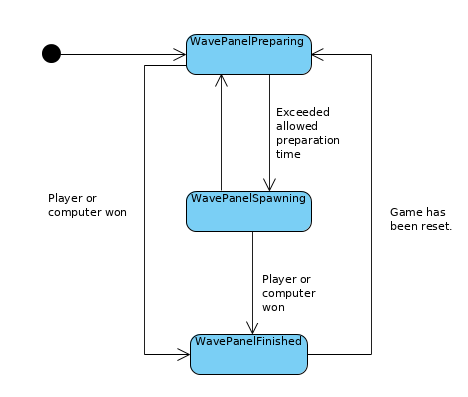
\includegraphics[scale=0.75]{res/wave-panel-states.png}
    \caption{Wave panel state transitions.}\label{fig:wavepanel-states}
\end{figure}



\newpage

\section{Design decisions}

discuss the motivation (arguments/reasons), consequences,
and alternatives for the decisions.
\newpage

\input{chapters/security-measures.tex}
\newpage

\section{Algorithm designs}
\newpage

\section{Non-functional requirements}
A few non-functional requirements have been identified. These requirements are explained below.

\textbf{The game should have no significant slowdowns} \newline
A game is not fun to play when it is not able to render quickly and at a consistent speed. Therefore the player should not encounter significant slowdowns while playing the game.

\textbf{The game should start up quickly} \newline
The game should launch within one minute, so that the player does not give up and play another game that does start up quickly.

\textbf{The UI should be intuitive} \newline
We don't want the user to have to read a large manual in order to be able to play the game. Therefore the User Interface should be intuitive, and if it's not intuitive the game should teach the player how to do a specific task.

\textbf{The game should be fun to play} \newline
While we understand that this is a vague non-functional requirement, we should always ensure that the game is fun to play. Due to time constraints we can't make the game as extensive as we would like, so we should focus on features that make the game fun to play.
\newpage
%----------------------------------

\bibliography{bib/sources}
\newpage

\section{Appendix}
\begin{figure}[!htb]
    \centering
    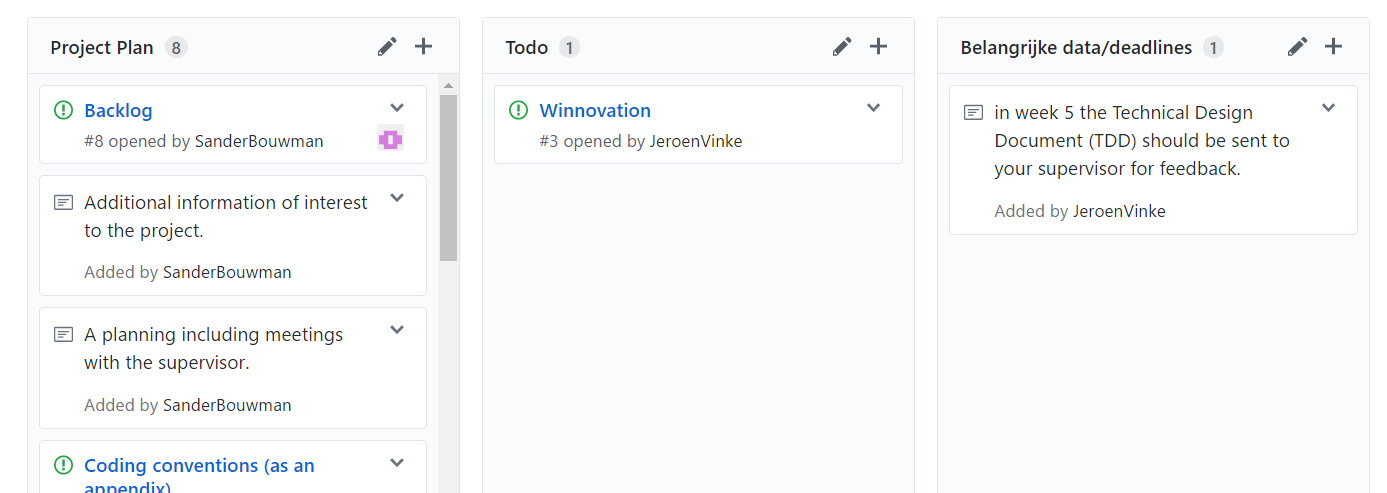
\includegraphics[angle=-90,origin=c,scale=0.75]
    {images/github-projects.PNG}
    \caption{GitHub project}\label{fig:githubproject}
\end{figure}

\end{document}
